
\section{Empirical Results}\label{sec:exper}




While we have shown mathematically that the ordering of compactness scores can be permuted by any map 
projection, the actual districts we wish to examine are relatively small compared to the surface of the Earth, 
and we might ask whether this order reversal actually occurs in practice.
We can extract the boundaries of the districts from a \textit{shapefile} from the U.S. Census Bureau\footnote{We use the U.S. Census Bureau's shapefile for the Congressional districts for the 115th Congress.} and compute the convex hull, Reock, and Polsby-Popper scores on the Earth and with respect to a common map projection\footnote{The code to compute the various compactness scores is based on Lee Hachadoorian's \textit{compactr} project. \cite{hachadoorian2018reock}} and examine the ordering of the districts with respect to both.

The projection we use is the familiar \textit{Mercator} projection, which is commonly used in settings like Internet mapping applications and pulldown maps in school classrooms.  
The Mercator projection presents latitudes and longitudes as equally-spaced horizontal and vertical lines, which causes small amounts of distortion near the equator, but large amounts outside of the tropics, with the areas of regions near the poles being dramatically inflated under the projection.








We observe overall that the orderings of districts under the Polsby-Popper score and convex hull score are relatively undisturbed compared to that of the Reock score.  This is because the \textit{values} of those scores do not change by too much under different projections.  Intuitively, this is because while both projections distort shapes, they do so in a way that does not affect either of these scores by too much. In the case of the Polsby-Popper score, the perimeter and area of the regions are changed in similar ways, and in the case of the convex hull score, the area of the convex hull of a region is distorted in the same way as the region itself. This leads to a similarity in the ratio of the areas of the districts across projections.

For regions in North America, such as our Congressional districts, the differences in the minimal bounding circle between the spherical and Mercator representation cause massive differences in both the raw values of the scores as well as the ordering.  The scores can change in either direction by upwards of $.1$ (recall that the value of the score is between zero and one) and there is almost no correlation in the ordering of the districts by their Reock scores on the sphere and under the Mercator projection. 

In \Cref{fig:reock_exp_tx}, we plot the ordering of the 36 Congressional districts of Texas under the Reock score as computed on the sphere and in the plane after applying the Mercator projection.  The rank on the sphere is along the horizontal axis and in the plane along the vertical axis.  Sweeping from left to right, one encounters the districts in order of least to most compact on the sphere and from bottom to top the least to the most compact in the plane.


		\begin{figure}[!h]
	\centering
	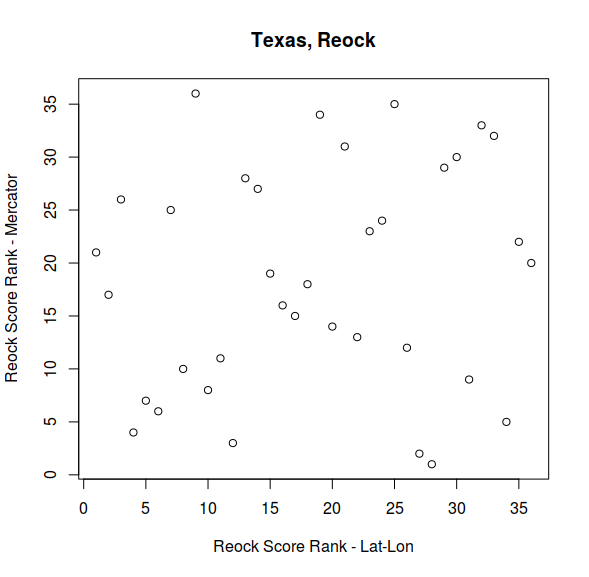
\includegraphics[width=.5\textwidth]{figs/texas_reock.png}

	\caption{The permutation of the Reock score ordering for Texas' Congressional districts.}
	\label{fig:reock_exp_tx}
\end{figure}

A perfect preservation of the order would result in these points all falling on the diagonal.  However, what we see in practice is that many points do lie near the diagonal but several are very far away, indicating a strong disagreement between the Reock ordering on the sphere and in the plane.  This effect is not a result of some idiosyncrasy of the shapes of Texas' Congressional districts.  We find similar effects for all other states with at least a moderate number of districts.

This suggests that while the convex hull,  Polsby-Popper, and Reock measures all share a similar mathematical flaw, in applications to Congressional redistricting, the manifestation of the permutation of the ordering of districts by their Reock score is quite dramatic and could have real consequences for parties trying to use this score to assess the geometric compactness of a districting plan.  While we are unable to find any court cases where the Reock score was used crucially to determine whether or not a plan was an illegal gerrymander, the state laws of Michigan do use a similar measure in their definition of compactness, where one similarly constructs the smallest bounding circle of a district but then excludes from that circle any area falling outside of the state before taking the ratio.\footnote{Michigan Comp. Laws \S 3.63}  For districts whose bounding circle falls entirely within the state, this definition aligns exactly with the Reock score, and so is similarly susceptible to this permutation effect of map projections.


